\documentclass{article}
\usepackage{leonine,amsmath,amssymb,amsthm,graphicx, setspace}%%xy, setspace, amscd (commutative diagram)
\title{Notes}

\author{Eric Purdy \footnote{Department of Computer Science,
    University of Chicago. Email: epurdy@uchicago.edu}}

%%\doublespace
\DeclareMathOperator*{\len}{len}
\newcommand\fakecite[1]{ {\bf [#1]} }

%% \newcommand\spk[2]{\includegraphics[width=#1mm]{images/#2.png}}
\newcommand\spk[2]{\framebox{images/#2.png}}

\begin{document}
\maketitle

\tableofcontents

\part{CURRENT WORK}

\section{Style Guide}

This is just a convenient reference for me as I try to keep all the
notation consistent and intuitive.

\bitem
\item Nonterminals: $X,Y,Z$ (use superscripts to enumerate)
\item Placed nonterminals: $X_{p,q}$
\item Start nonterminals: $S,T$
\item Terminal: $\ell$
\item Placed terminal: $\ell_{p,q}$
\item Curves: $A,B,C, C_n$
\item Points: $c_i$
\item Curvilinear forms: $\lambda, \mu, \nu$ ($\sigma$ for starting)
\item Grammars: $\GGG, \HHH$
\item Set of nonterminals: $\NNN$
\item Set of starting nonterminals: $\SSS$
\item Set of rules: $\RRR, \RRR(X)$
\item Set of midpoint distributions: $\MMM$
\item Set of rule-choice distributions: $\XXX$.
\item Do we want to differentiate open/closed curves notationally?
$ST$ vs. $\overline{ST}$ is reasonable, if so.
\eitem

\section{Grammatical Curve Models }

Pedro's hierarchical curve models for curve classification

\subsection{The Task}

We want to build a system that can classify curves. We will give it a
set of curves from $n$ different classes $C_1,\dots,C_n$, and we wish
to assign new curves to the class that they most belong in. Some
datasets for this task are:
\bitem
\item Swedish Leaf dataset. Here we are given the silhouettes of
  leaves from fifteen different species of tree. (Species include
  maple, oak, and some sort of willow.) For each class, we are given
  25 example leaves, and then we want to build a classifier that will
  accurately classify another 50 examples from each species.

\item MPEG7.

\eitem

Our generic approach to this task will be to build a probabilistic
model for each class. Given a novel curve $x_*$, we will compute $\PP(
x_* \mid C_i)$ for each class and assign $x_*$ to the class which
gives it the highest likelihood.

\subsection{Some Motivation}

To motivate our discussion of curve grammars, we will first give an
amusing example of such a grammar, which is inspired by L-systems. A
Lindenmayer system, or L-system, is a parallel string rewriting
system. Although they are defined on strings, it is popular to render
their output as a picture using a ``turtle language'' akin to
Logo. They are a simple and intuitive way to generate fractal
images. Since our formalisms do not match up perfectly with the usual
definition of L-systems, we will not discuss them.

We will informally discuss curve rewriting systems, where we
iteratively replace straight lines with curves composed of straight
lines. We will represent our curves like this: \spk{10}{gline}, so that
we remember which endpoint is which.

Consider the following system\footnote{generated by $A=A+A+A--$ with
  angle $60^\circ$ in Inkscape}:
$$ \spk{10}{gline} \to \spk{10}{gbump} .$$

Applying this rule a few times, we generate \spk{10}{gline}, \spk{10}{gbump},
\spk{10}{gbump2} and \spk{15}{gbump3}.

%% An L-system might represent
%% this rewrite rule as $A\to A+A+A$. Here, if we interpret the symbol
%% $A$ as ``go forward one step'' and the symbol $+$ as ``rotate 60
%% degrees to the left'', then a turtle following the directions $A+A+A$
%% would generate the curve 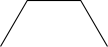
\includegraphics[width=10mm]{bump.png},
%% suitably rotated.

We now wish to construct a more complicated system. We need to start
distinguishing different kinds of curves, in this case \spk{10}{gdash}
versus \spk{10}{gline}. Consider the following system\footnote{generated by 
$A=B+A+B; B=A-B-A$ with angle $60^\circ$ in Inkscape}
\begin{align*}
\spk{15}{gline} &\to \spk{15}{gBAB} \\
\spk{15}{gdash} &\to \spk{15}{gABA}.
\end{align*}

If we start from \spk{10}{gline}, we successively generate
\spk{10}{gBAB}, \spk{20}{gsier2}, and \spk{20}{gsier3}.  Suprisingly,
after a large number of iterations, a pattern arises that may be
familiar: Sierpinski's triangle! After eight iterations, we have
(filling in the dashed lines for simplicity) curve $C$:

\spk{100}{gsier8}.

These curves were generated by Inkscape's L-system function, which has
a randomizing option. It is interesting to randomize the last
example. Here is the randomized version $C'$ I got, with fairly little
noise (10\% randomization in the length of line segments, and 5\%
randomization in the angles. These parameters only make sense in a
more standard L-system framework):

\spk{100}{gbadsier}.

This has no global similarity at all to the other curve! Inkscape is
using a Markov-like source of randomness, and little errors at the
local level add up to huge changes at the global level. If we are
going to have a statistical model for perceptual similarity of curves,
we will have to find a way to introduce long-range dependencies. This
brings us to our next section: probabilistic context-free grammars on
curves.

\subsection{Model: PCFG's on Curves}

Our probabilistic models will be probabilistic context-free grammars.
We define a Probabilistic Context-Free Grammar framework for
generating and parsing one-dimensional curves in a two-dimensional
space.

We will represent a curve as a sequence of oriented line segments. We
will denote a line segment going from points $p$ to point $q$ by
$\ell_{p,q}$. A curve will then have the form
$$ \ell_{p_0,p_1} \ell_{p_1,p_2}\cdots \ell_{p_{n-1},p_n},$$ and
$p_0$ will be equal to $p_n$ iff the curve is closed.  For a closed
curve, this sequence is circular, and we consider any cyclic
permutation of the line segments to be the same curve.

Analogously to context-free grammars over strings, we introduce
non-terminals. Our non-terminals will represent oriented curves
(either open or closed) whose endpoints are fixed, but whose path
between those endpoints is unspecified. We denote such a non-terminal
of type $N$ going from point $p$ to point $q$ by $N_{p,q}$. By itself,
$N$ will denote a type of non-terminal that can be instantiated
between any $p$ and $q$.

\begin{defn}
A {\em curvilinear form} (by analogy with a sentential form for string
grammars) is a sequence of oriented sub-curves denoted by
non-terminals. It will have the form
$$ \alpha^{(0)}_{p_0,p_1} \alpha^{(1)}_{p_1,p_2} \cdots
\alpha^{(n-1)}_{p_{n-1},{p_n}}$$ where each $\alpha^{(i)}$ can be
either $\ell$ or any non-terminal type. As with curves, $p_0$ will be
equal to $p_n$ iff the curvilinear form is closed.

We will also have {\em abstract curvilinear forms} which have no
associated geometric information. They will have the form
$$ \alpha^{(0)} \alpha^{(1)} \cdots \alpha^{(n-1)}.$$ We will specify
whether these are open or closed, since there is no way to
tell. Again, closed abstract curvilinear forms will be invariant under
cyclic permutations.
\end{defn}

We next introduce substitutions and substitution rules, which allow us
to transform curvilinear forms, ultimately producing curves. We will
perform substitutions of the form
$$ A_{p,q} \to B^{(1)}_{p,p_1} B^{(2)}_{p_2,p_3} \cdots
B^{(k)}_{p_k,q}.$$ Since $A_{p,q}$ represents an unspecified path from
$p$ to $q$, substitution simply gives a more specific route, in terms
of which points we will visit in between (the $p_i$, which we will
call ``control points'') and what sort of path we will follow between
these points (the $B^{(i)}$).

In order to give a substitution rule for performing substitutions, we
need to give
\bitem
\item An {\em abstract substitution rule} $A\to B^{(1)}\cdots B^{(k)}$.
\item a rule for determining the $p_i$ in terms of $p$ and $q$.
  \eitem

In order to make the rules be context-free, we would like the specific
path followed by $A_{p,q}$ (i.e., the $p_i$) to be independent of the
context in which $A_{p,q}$ occurs (i.e., $p$ and $q$), given that we
are taking this particular path. Accordingly, we specify the $p_i$ in
the coordinate system $\CCC(p,q)$ that maps $(0,0)$ to $p$ and $(1,0)$
to $q$.

In practice, applying a substitution rule is problematic because the
$p_i$ live in an infinite domain ($\RR^2$), but we want to deal with
curves that (1) live in a finite domain (the pixels of the image
plane) and (2) are expected to exhibit a good deal of variation. Thus,
we give a distribution over the $p_i$ called the control-point
distribution:
$$ \PP \left[ p_1,\dots, p_k \mid p,q \right] = \mu_{A\to
  B^{(1)}\cdots B^{(k)}}(p_1,\dots, p_k ; p,q).$$ Because we want a
context-free formulation, we will restrict the control-point
distribution to be of the form
$$ \PP \left[ p_1,\dots, p_k \mid p,q \right] = \mu_{A\to
  B^{(1)}\cdots B^{(k)}}( \widehat{p}_1, \dots, \widehat{p}_k)$$ where
$\widehat{p_i}$ are the coordinates of $p_i$ in $\CCC(p,q)$.

\begin{defn}
A probabilistic context-free shape grammar (PCFSG) is a tuple 
$\GGG = (\NNN, \RRR, \SSS, \ell, \MMM, \XXX)$, where
\bitem
\item $\NNN$ is a set of curve types
\item $\RRR$ is a set of abstract substitution rules
\item $\SSS$ is a set of starting curvilinear forms
\item $\ell \in \NNN$ is a curve type representing a line segment
\item $\XXX = \{\rho_X \mid X\in \NNN, X\ne \ell\} \cup
  \{\rho_\SSS\}$, where $\rho_X$ is a probability distribution over
  $\RRR(X)$, and $\rho_\SSS$ is a distribution over $\SSS$
\item $\MMM = \{ \mu_{X\to Y^{(1)}\cdots Y^{(k)}} \mid (X\to
  T^{(1)}\cdots Y^{(k)}) \in \RRR\}$ is a set of control-point
  distributions.
\eitem
\end{defn}

\mar{Update informal sampling for starting forms formulation}
We sample from a curve PCFG by starting with $S_{p,q}$ for arbitrary
$p$ and $q$, and, while there is a subcurve $A_{p,q}$ in our
curvilinear form, with $A\ne \ell$, picking a random substitution rule
$A \to B^{(1)} \dots B^{(k)}$ according to $\rho_A$, and picking
random control points $p_1,\dots, p_k$ according to $\mu_{A\to
  B^{(1)}\dots B^{(k)}}$.

There is a slight difficulty here in that we cannot define the
control-point distribution if $p$ and $q$ are equal. This is
important, since we are mainly interested in closed curves, so we
would like to start with $S_{p,p}$ for some arbitrary $p$. In this
case, we define a probabilistic context-free grammar over closed
curves by having two start symbols $S$ and $T$, and starting with the
curvilinear form $S_{p,q} T_{q,p}$ for an arbitrary choice of $p$ and
$q$.

\subsection{Our Model for Curves}

For simplicity and efficiency, we will usually restrict our
substitution rules to be of two forms:
\bitem
\item Binary rules of the form $$ A_{p,q} \to B_{p,r} C_{r,q}.$$ We
  will call the point $r$ the midpoint instead of a control point.
\item Rules of the form $$ A_{p,q} \to \ell_{p,q}.$$
\eitem 

We will model the midpoint distribution using the complex Watson
distribution, defined as follows: consider our points in $\RR^2$ as
complex numbers, and let $\tilde{z} = \left(\begin{array}{c c c} p& r&
  q\end{array}\right)$.  Let $\tilde{\mu} = \left(\begin{array}{c c c} p&
    \widehat{r} & q\end{array}\right)$, where $\widehat{r}$ is the
    most likely value of $r$. For various reasons, we will multiply
    $\tilde{z}$ by the $2\times 3$ Helmert matrix
$$H = \left(\begin{array}{c c c} 1/\sqrt{2} & -1/\sqrt{2} & 0
  \\ 1/\sqrt{6} & 1/\sqrt{6} & -2/\sqrt{6}\end{array}\right), $$ and
then normalize the result to get our coordinates:
\begin{align*}
\langle p, q, r\rangle = z &= H\tilde{z} / \|H\tilde{z}\| \\
\mu &= H\tilde{\mu} / \|H\tilde{\mu}\|
\end{align*}

Then
$$\mu_{A\to BC}(r) = Watson(\mu,\kappa) =
\frac{1}{Z(\kappa)}e^{-\kappa |z^*\mu|^2},$$ where $\kappa$ is a
concentration parameter. More details on the Watson distribution can
be found in Mardia and Dryden.

\subsection{Defining a Parse and Writing the Likelihood}

Let $G$ be a shape grammar in Chomsky Normal Form, and let
$C$ be a curve of length $n$.

A parse of $C$ using $G$ is a tree $T=(V,E)$, where
$V = V_{\ell} \cup V_{bin} \cup V_{lex}$. The interior
nodes of $T$ are in $V_{bin} \cup V_{lex}$, and each is
labeled by a triplet $(X,i,j)$ where $X\in N(G)$, 
$1\le i,j \le n$. The leaf nodes of $T$ are 
exactly $V_\ell$, and they are all labeled by $\ell$.

The nodes in $V_{bin}$ are called binary nodes, and always
have two children. If $(X,i,j)\in V_{bin}$ , its two 
children must be labeled with $(Y,i,k)$ and $(Z,k,j)$
for some $k\in [n]$ and 
some $Y$ and $Z$ such that $X\to YZ$ is 
a rule of $G$. In this case, we
 will let $rhs( (X,i,j) ) = BC$, and $ch( (X,i,j) ) = \{(Y,i,k), (Z,k,j)\}$.

The nodes in $V_{lex}$ are called lexical nodes. They each
have one child, which is a leaf node.
In this case, we will let $rhs( (X,i,j) = \ell$.

Then 
\begin{align*}
P(C\mid G) = \sum_{T} &\prod_{\substack{v=(X,i,j) \in V_{bin}, \\ch(v)=\{(Y,i,k),(Z,k,j)\}}}
  \mu_{X\to YZ}(c_i, c_k, c_j) \cdot \\
&\prod_{(X,i,j) \in V_{bin} \cup V_{lex}} p_G(X \to rhs( (X,i,j) )
\end{align*}

Note that, for a closed curve, the top-level rule has no geometric
information. For simplicity, we can assume that $\mu_{\ \to ST} \equiv 1$.

\subsection{Defining a Parse and Writing the Likelihood 2}

Let $\GGG = (\NNN,\RRR,\SSS,\ell,\MMM)$ be a shape grammar in Chomsky
Normal Form, and let $C$ be a curve of length $n$.

A $\GGG$-parse of $C$ is a directed tree $T=(V,E)$, where $V=V_{NT}
\cup V_\ell$.  $V_{NT}$ contains the interior nodes of $T$, each of
which is labeled by $X_{c_i c_j}$ for some $X\in \NNN$, $i,j\in
[n]$. $V_\ell$ contains the leaf nodes of $T$, each of which is
labeled by $\ell_{c_i c_{i+1}}$ for some $i$. Every segment $\ell_{c_i
  c_{i+1}}$ is used exactly once as a label.

$V_{NT} = V_{bin} \cup V_{lex}$. If $X_{c_i c_j}\in V_{bin}$ , then
$X_{c_i c_j}$ has two children, $Y_{c_i c_k}$ and $Z_{c_k c_j}$, where
$[X\to YZ] \in \RRR$. We will set $rhs(X_{c_i c_j})=YZ$.  We will let
$R(T) = \{ [X\to YZ]_{c_i c_j c_k} \mid X_{c_i c_j} \sim Y_{c_i c_k},
Z_{c_k c_j}\}$.

If $X_{c_i c_j}\in V_{lex}$, then $X_{c_i c_j}$ has one child $v\in
V_\ell$. In this case, we will set $rhs(X_{c_i c_j})=\ell$.

Let $Parse_\GGG(C)$ be the set of all $\GGG$-parses of $C$.  The
likelihood of $C$ according to $\GGG$ is
\begin{align*}
P(C\mid\GGG) &= \sum_{T\in Parse_\GGG(C)} P(C,T\mid G)\\
&= \sum_{T\in Parse_\GGG(C)} P(C\mid T, G) P(T\mid G)\\
\end{align*}

$$P(C\mid T,\GGG) = \prod_{[X\to YZ]_{pqr}\in R(T)} \mu_{X\to YZ}(p,q,r)$$
$$P(T\mid \GGG) = \prod_{X_{c_i c_j}\in V_{NT}} \rho_{X}(rhs(X_{c_i c_j}))$$

\subsection{Parsing Algorithm}

In order to classify curves, we need to be able to compute the
likelihood of a curve given a grammar. As an approximation, we can
compute the probability of the most probable parse of that curve. We
call this the Viterbi parse.

Calculating the probability of a curve involves either summing or
maximizing over the various ways to decompose each curve into two
subcurves by picking a midpoint. This can be done via dynamic
programming.

We are using two different parsing algorithms: an adaptation of the
CKY algorithm (for finding the probability of the Viterbi parse), and
an adaptation of the inside-outside algorithm (for finding the true
probability). Both algorithms must be adapted because we are
ultimately parsing circular strings, so we have to consider the
possibility that a given nonterminal maps to a subset of the curve
that wraps around the end of the curve.

This is fairly straightforward.


\section{Discretizing for Efficiency}

In order to speed up the algorithm, we approximate each curve with
polygonal segments.  Current behavior is to pick a desired final curve
length $L$ (our default it 40 points), and try to simultaneously not
deviate from that and approximate the curve well. We do this by
minimizing:

$$\argmin_{ \{n_i \} } \sum_i \sum_{j=0}^{\ell_i} \left\| p_{n_i+j} -
\left( \frac{\ell_i - j}{\ell_i} p_{n_i} + \frac{j}{\ell_i}
p_{n_{i+1}} \right) \right\|^2 + \lambda \sum_i (\ell_i -
\hat{\ell})^2,$$
  
where $\ell_i$ is the length of the $i$-th segment and $\hat{\ell} =
N/L$ is the ideal segment length to go from $N$ points to $L$
points. Note that $p_{n_i + j}$ wraps around: $p_{n_i + j} = p_{n_i+j
  \mod N}$ . I have been using $\lambda=1$. The segmentation algorithm
is not particularly sensitive to $\lambda$.

This minimization is done with a straightforward dynamic program.

\section{A Prior over Models}


We need to give both a prior over the structure of the grammar, and over
the parameters $\{\rho_A\}$ and $\{\mu_{A\to BC}\}$.


\subsection{Prior over Structure}

We are using a minimum description length prior for the structure of
the grammar. That is, we set $P(G) = \frac{1}{Z} e^{-len(enc(G))}$ for
some encoding function $enc(\cdot)$.  The only parts of the grammar
structure that we need to encode are $\NNN$, the set of curve types,
and $\Pi$, the set of abstract substitution rules. For $\NNN$, we only
need to know $n = |\NNN|$, since we can just enumerate $\NNN$ and
refer to each curve type by an integer between $1$ and $n$. This
requires $\log(n)$ bits.

We encode each element $A\to BC$ or $A\to \ell$ of $\Pi$ as either
$$ 1\ id_A\ id_B\ id_C$$
or
$$ 0\ id_A, $$
respectively.  Specifying an id takes $\log(n)$ bits, so we require
$3\log(n) + 1$ bits to encode the first sort of rule, and $\log(n) +
1$ bits to encode the second sort of rule.

Thus our total description length is

\begin{align*}
&\log(n)  \\
+& (3\log(n) + 1)  \times \#[\text{binary productions}]\\
+& (\log(n) + 1) \times \#[\text{lexical productions}] .
\end{align*}

\subsection{Prior over Parameters}
\label{sec-prior-param}

We must specify a prior for the $\mu_{X\to YZ}$ and $\rho_X$.  For
optimal results, we tailor the specific prior to the scale $s$ of the
subcurve we are modeling, where $s(C') = \frac{|C'|}{|C|}$.

Let $X\in \NNN$. Let $s$ be our scale parameter. We let
$$\rho_X \sim Dir(\alpha_1, \dots, \alpha_k),$$
where
\begin{align*}
\alpha_1 &= \alpha_{dir} e^{- \alpha_{\rho} s^2} \\
\alpha_i &= \alpha_{dir} \frac{1 - e^{- \alpha_{\rho}s^2}}{k-1}, 2\le i\le k
\end{align*}
where $\alpha_1$ corresponds to the rule $X\to \ell$.
Currently $\alpha_{dir} = 10.0$, $\alpha_\rho = 1000.0$.

Let $X\to YZ$ be a rule of $G$. Let $s$ be our scale parameter.  We
set $\mu_{X\to YZ}$ equal to a Watson distribution with random mode $\mu$ and
random concentration $\kappa$, where
$$\kappa \sim Gamma(\sigma, \theta=\bar{\kappa}/\sigma)$$
$$\mu \sim Watson(\mu_0, \alpha_{mp} \kappa)$$
where $\sigma$ is the shape parameter of the Gamma distribution, and
$\bar{\kappa} = \alpha_{\kappa} s$. 

Currently $\sigma=5$, $\alpha_\kappa = 4000.0$. $\alpha_{mp}$ is a
parameter dictating the balance between prior and observation.  We
choose $\mu_0$ to correspond with the mean of the two endpoints.

\section{Learning Parameters}

There are two components to our model: the structure of the grammar,
and the value of the continuous parameters. If we have an appropriate
structure, learning the continuous parameters can be done using the EM
algorithm, modified so as to take priors into account.

Doing the full EM algorithm would require us to sum over all possible
parses. For the sake of simplicity and efficiency, we approximate this
by only using the parse with highest likelihood, called the Viterbi
parse.

In this section we give approximations to the maximum a posteriori
setting of the parameters given observed data. Let $C_1, \dots, C_n$
be our observed curves, $\GGG$ be our grammar (whose structure is
fixed), and let $T_i$ be the Viterbi parse tree of $C_i$ according to
$\GGG$.

\subsection{Multinomial Distribution}

We want to estimate the distribution $\rho_X$, which is distributed
according to some $Dir(\alpha_1, \dots, \alpha_m)$. For each of the
rules $X\to \lambda$, we have a count $k_i$ of how many times that
rule appears in the $T_j$. The maximum a posteriori estimate of
$\rho_X$ is then a multinomial with probabilities 
$$p_i = \frac{k_i + \alpha_i - 1}{\sum_i k_i + \sum_i \alpha_i - m}.$$

\subsection{Watson Distribution}

We wish to estimate $\mu_{X\to YZ}$, given the parses $T_1, \dots,
T_n$. For each time the rule $X\to YZ$ was used, we observe one
midpoint. Transforming these into our preferred coordinates, we get
observations $z_1, \dots, z_m$. We wish to use the $z_i$ to estimate
the parameters $\mu$ and $\kappa$ of our Watson distribution.

Let $\alpha_{mp}, \mu_0$ be defined as in Section
\ref{sec-prior-param}. Let $\gamma(\kappa;\sigma,\theta) = \log
Gamma(\kappa; \sigma,\theta)$.  Let $c(\kappa)$ be the normalizing constant
of the Watson distribution.

\begin{align*}
P(\mu, \kappa \mid z_1,\dots,z_m) &\propto
P(\mu, \kappa) P(z_1,\dots,z_m\mid \mu, \kappa) \\
&= \exp[ \alpha_{mp}\kappa \mu^* \mu_0 \mu_0^* \mu
- \log c(\alpha_{mp} \kappa) + \gamma(\kappa; \sigma,\theta)
+ \kappa \sum_i \mu^* z_i z_i^* \mu - m \log c(\kappa)
\\
&= \exp[
\kappa \mu^* (\alpha_{mp} \mu_0 \mu_0^* + \sum z_i z_i^*)\mu
- \log c(\alpha_{mp} \kappa) - m \log c(\kappa) + 
\gamma(\kappa; \sigma, \theta) ]\\
\log P(\mu, \kappa \mid z_1,\dots,z_m) &= 
c_{norm} + 
\kappa \mu^* (\alpha_{mp} \mu_0 \mu_0^* + \sum z_i z_i^*)\mu
- \log c(\alpha_{mp} \kappa) - m \log c(\kappa) + 
\gamma(\kappa; \sigma, \theta) \\
&= c_{norm} + 
\kappa \mu^* A \mu
- \log c(\alpha_{mp} \kappa) - m \log c(\kappa) + 
\gamma(\kappa; \sigma, \theta),
\end{align*}

where $A = \alpha_{mp} \mu_0 \mu_0^* + \sum z_i z_i^*$.
Since $\mu$ only appears in the term $\kappa \mu^* A \mu$,
and $A$ has non-negative eigenvalues, it is clear
that we maximize the posterior by choosing $\mu$ to be
the dominant eigenvector of $A$.
Let $\lambda_{\max}$ be the associated eigenvalue. Then

\begin{align*}
\log P(\mu, \kappa \mid z_1,\dots,z_m) &= 
c_{norm} + \kappa \lambda_{\max}(A) - 
\log c(\alpha_{mp} \kappa) - m \log c(\kappa) + 
\gamma(\kappa; \sigma, \theta)\\
\end{align*}

Taking partial derivatives, and using the approximation
$c(\kappa) = 2 \pi^2 \frac{1}{\kappa} e^\kappa$,
we arrive at the approximate solution

$$
\frac{\partial \log P(\mu, \kappa \mid, z_1,\dots,z_m)}
{\partial \kappa} = 
\lambda_{max} - \alpha_{mp} -m + \frac{1+m}{\kappa} + 
\frac{\sigma-1}{\kappa} - \frac{\sigma}{\bar{\kappa}} = 0
$$
$$
\widehat{\kappa} = \frac{\sigma+m}{\frac{\sigma}{\bar{\kappa}}
+ m + \alpha_{mp} - \lambda_{max}}
$$

$$
\widehat{\mu} = \mbox{ dominant eigenvector of }
A\mbox{, where } A = \alpha_{mp} \mu_0 \mu_0^* + \sum z_i z_i^*
$$

Examining this solution, we see that our estimate of the
midpoint is similar to the maximum likelihood estimate of
a Watson distribution, but is adapted to contain
$\alpha_{mp}$ artificial observations at the prior mode.

The posterior estimate of the concentration will be at
a maxmimum when all $z_i$ are identical and equal to 
$\mu_0$. In this case, $\lambda_{max}$ will be
$m + \alpha_{mp}$, and $\widehat{\kappa} = 
\bar{\kappa} \frac{\sigma+n}{\sigma}$. Thus, our concentration will
increase essentially linearly with the number of examples, but will never
be infinite.

In general, the $z_i$ and $\mu_0$ will be more spread out, causing $A$
to have a lower dominant eigenvalue, and lowering the concentration.

\section{Learning the Model Structure}

\subsection{Building a Grammar from a Single Curve}
 
This work is based on a nearest-neighbor algorithm. The grammar we
build initially emulates the matching procedure used there. We will
build a grammar from each training example, which generates curves
that look like that specific example.

We construct a grammar $\GGG$ from a curve $C$ by first choosing a
parse of $C$, and then giving $\GGG$ the necessary nonterminals and
rules. We use this parse to set the continuous parameters of the
grammar according to the formulas given in the previous section.

Let $p_1,\dots,p_n$ be the points of $C$. Note that $C$ is closed, so
that there is a line segment from $p_n$ to $p_1$. For notational
convenience, we will let $p_0 = p_n$.

We then hierarchically decompose $C$ by splitting it into two open
curves
$$p_0,\dots,p_k$$
and
$$p_k, \dots, p_n.$$ 
We add nonterminals $N^{0k}, N^{kn}$ to $\NNN$, and we let $\SSS = \{
N^{0k} N^{kn} \}$ be the set of starting forms.  We can choose
$k=\lfloor \frac{n}{2} \rfloor$. Later, we will look at other options.
%% Currently we just use $k={\lfloor \frac{n}{2}
%%   \rfloor}$, i.e., we split the initial curve into two curves of equal
%% length. We could probably do better by choosing the split more
%% intelligently.

We then recursively break each curve $p_i,\dots,p_j$
into two subcurves 
$$p_i, \dots, p_k$$
and
$$p_k, \dots, p_j.$$ 
(Note that the midpoint of the larger curve is always shared by the
two subcurves.)  We add nonterminals $N^{ik}, N^{kj}$ to $\NNN$, and
add the rule $N^{ij} \to N^{ik} N^{kj}$ to $\RRR$.  We can choose
$k=\frac{i+j}{2}$. Later, we will look at other options.
%% Here we choose
%% $k=\frac{i+j}{2}$. We could probably do better by choosing the split
%% more intelligently.

When we see a curve of length one, $p_i,  p_{i+1}$, we add the rule
$N^{i i+1} \to N^{i i+1} N^{i i+1}$ to $\RRR$. (This allows our grammar
to model curves which are longer than $C$.)

Finally, for every $N^{ij} \in \NNN$, we add a rule $N^{ij} \to \ell$.
(This produces the bottom-most level of $C$ when $j=i+1$. When $j\ne
i+1$, this allows our grammar to model curves which are shorter than
$C$.)

To give an initial estimate for the continuous parameters, we use
$$s = \frac{j-i}{n},$$
$$\mu_{ N^{ij} \to N^{ik} N^{kj} } = Watson(\langle p_i, p_k,
p_j\rangle, \alpha_\kappa s),$$
$$\rho_{N^{ij}} (N^{ij}\to \ell) = e^{- \alpha_\rho s^2},$$
$$\rho_{N^{ij}} (N^{ij}\to N^{ik}N^{kj}) = 1 - e^{-\alpha_\rho s^2}.$$

%% Given this hierarchical decomposition, we define a grammar as follows:
%% for every subcurve $p_i,\dots,p_j$ in the decomposition, we create a
%% new nonterminal $N^{ij}$ that is responsible for generating only that
%% subcurve.  If $p_i,\dots,p_j$ was broken into $p_i,\dots, p_k$ and
%% $p_k,\dots,p_j$ when we were creating the decompostion, we introduce a
%% rule $N^{ij} \to N^{ik} N^{kj}$. We need to specify the midpoint
%% distribution of this rule: we use a complex Watson distribution with
%% mode equal to the point $p_k$ when represented in the coordinate frame
%% where $p_i$ is mapped to $(0,0)$ and $p_j$ is mapped to $(1,0)$.

%% We still need to specify a concentration for the Watson
%% distribution. It is meaningless to estimate a variance parameter from
%% a single data point, so we use $\kappa = 1000 \cdot (j-i)$ as a
%% heuristic. Choosing a concentration proportional to arclength is
%% motivated by the model of \fakecite{hier}.

%% We want our grammar to be able to produce both longer and shorter
%% curves. To this end, we introduce two new kinds of rules. For every
%% nonterminal $N^{ij}$ we introduce the rule $N^{ij} \to \ell$, so that
%% any subcurve in our hierarchical decomposition can be mapped to a
%% single line segment. This allows the grammar to model curves that are
%% shorter than our original curve.

%% To model longer curves, for each nonterminal $N^{i\ i+1}$ we introduce
%% a recursive rule $N^{i\ i+1} \to N^{i\ i+1} N^{i\ i+1}$. We use the
%% complex Watson distribution for the midpoint, with mode equal to
%% $(\half,0)$ (i.e., the mean of the two endpoints) and
%% concentration $\kappa = 1000$.

%% There is only one more kind of parameter to specify, which is the
%% relative probability of the rules
%% \begin{align*}
%% N^{ij} &\to N^{ik} N^{kj} \\
%% \intertext{and}
%% N^{ij} &\to \ell \\
%% \intertext{ and the relative probability of the rules}
%% N^{i\ i+1} &\to \ell \\
%% \intertext{and}
%% N^{i\ i+1} &\to N^{i\ i+1} N^{i\ i+1}. \\
%% \end{align*}

%% As a heuristic, we set $P(N \to \ell) = e^{-1000 \frac{(j-i)^2}{n^2}}$
%% (with $j=i+1$ in the second case).




\subsection{Optimizing the Grammar from a Single Curve}

When constructing a grammar from a single curve, we have a choice in
how we split the curve each time. It is straightforward to do this in
such a way that we optimize the prior probability of the resulting
grammar. In practice, this means mainly choosing the midpoints to make
the subcurves straight, and the two subcurves of roughly equal length.


This is done via dynamic programming.
\mar{Explain!}


\subsection{Merging the Leaves}
We will usually merge all nonterminals that are ``leaves'', i.e.,
those nonterminals $N$ whose only expansions are $N\to NN, N\to \ell$.
\mar{Explain!}

\subsection{Building a Grammar from Multiple Curves by Greedy Optimization}

It is a well-defined question to ask for the shape grammar structure
and parameters which give us the maximum posterior for a set of
training examples given our chosen prior and likelihood
models. Unfortunately, we do not know how to optimize over all grammar
structures, and we do not know how to optimize over even restricted
classes of grammars efficiently. Here we describe a restricted class
of grammars and a greedy approach to finding a reasonable structure.

\subsubsection{Incremental Incorporation}

Suppose that we have a grammar $G_n$ which is an acceptable
explanation of example curves $C_1,\dots, C_n$.  Among the restricted
class of grammars we are examining, we wish to pick the best grammar
$G_{n+1}$ to explain $C_1,\dots, C_{n+1}$. To make the problem more
tractable, we will use the Viterbi approximation, and we will only
look at $G_{n+1}$ which contain all nonterminals and rules of $G_n$.

Because of the greedy search strategy, it seems sensible
to choose our next curve $C_{n+1}$ to be the next unexplained
curve which is least likely under $G_n$. Hopefully, this will
allow us to discover all the necessary structure quickly.

We simplify matters by only considering single-use grammars.
\begin{defn}
A {\em single-use grammar} is one in which every nonterminal $N\in
\NNN$ appears on the right-hand side of at most one rule, and in which
the start nonterminal(s) do not appear on the right-hand side of any rule,
and the starting form does not contain any nonterminal twice.
\end{defn}
\mar{Have to allow $L\to LL$}
\mar{appears only once on right hand side, also}
\mar{$\Pi(X)$ is set of rules with $X$ on the left hand side}

\begin{defn}
For a curvilinear form $\Phi = \phi_1 \cdots \phi_k$, and a
closed-curve grammar $G = (\NNN,\Pi,S,T,\ell)$, let $$SUB_G(\Phi) = \{
r_1(\phi_1) \cdots r_k (\phi_k),\mid r_i \in \Pi(\phi_i) \}.$$ A derivation is
a list of curvilinear forms $\Phi_1,\dots, \Phi_k$, where $\Phi_1 =
ST$, $\Phi_k = \ell^n$, and $\Phi_{i+1} \in SUB_G(\Phi_i)$ for $1\le i
< k$.
\end{defn}

\begin{lem}
Any derivation from a single-use grammar $G$ uses each nonterminal at
most once. 
\end{lem}
\begin{proof}
Let $D = (\Phi_1, \dots, \Phi_k)$ be a derivation from $G$.  Suppose
that $\Phi_h$ and $\Phi_{h'}$ contain the same symbol $N$, where $h$
is minimal. $N$ appears on the right hand side of only one rule,
without loss of generality $r : X \to N Z$. Then, if $h>1$, $X$ must
occur in both $\Phi_{h-1}$ and $\Phi_{h'-1}$, contradicting the
minimality of $h$. If $h=1$, $N$ is one of the start nonterminals, so
$G$ should not have such a rule $r$.

Suppose that $\Phi_h$ contains some nonterminal $N$ twice, where $h$
is minimal. Then, if $h>1$, we can again find the unique $r : X \to N
Z$ with $N$ on the right-hand side. Then $X$ must appear twice in
$\Phi_{h-1}$, contradicting the minimality of $h$. If $h=1$, then the
starting form of $G$ contains a repeated nonterminal, which is not
allowed.
\end{proof}


\subsection{Almost Single Use Notes}

\begin{defn}
A grammar $\GGG$ is {\em almost single-use} if $\NNN = \NNN_{NT} \cup
\NNN_{PT}$, with the following conditions:
\bitem
\item If $X\in \NNN_{NT}$, then $X$ appears at most once on the right
  hand side of at most one rule in $\RRR$, or appears at most once in
  at most one starting form in $\SSS$, but not both.
\item If $X\in \NNN_{PT}$, then $X$ appears in a rule $X\to XX$. $X$
  appears at most once on the right hand side of at most one other
  rule in $\RRR$, or at most once in at most one starting form in
  $\SSS$, but not both. Also, $X$ is on the left side of exactly two
  rules, $X\to XX$ and $X\to \ell$.
\eitem
\end{defn}

We are searching over this space, while requiring that $X\to XX$ rules
have a flat midpoint.

\begin{lem}
Let $\GGG$ be an almost single-use grammar, $C$ a curve, and $T$ a
parse tree. Then, if $X\in \NNN_{NT}$, there is at most one $X_{pq}$
in $V$. If $X\in \NNN_{PT}$, then vertices of the form $X_{pq}$ form a
single subtree of $T$.
\end{lem}
\begin{proof}
First part is same as before.

Second part: Since $X\to XX$ and $X\to \ell$ are the only
substitutions for $X$, it is clear that all descendants of $X_{pq}$
will be either $X_{p'q'}$ or $\ell$. Thus, we need only prove that
there is at most one such subtree. Consider the set of $X_{pq}$ whose
parent is not of the form $X_{p'q'}$, and suppose that there are at
least two. Recall that $X$ appears on the right hand side of only two
rules, $X\to XX$ and $Z\to XY$. Furthermore, $Z\notin \NNN_{PT}$, since
$Z\to XY$ is not of the form $Z\to ZZ$. Thus, we will have two
occurrences of $Z$, but $Z\notin \NNN_{PT}$, and the first part of the
lemma is violated for $Z$.
\end{proof}


%% The parse of $C_{n+1}$ under $G_{n+1}$ will be a parse tree labeled
%% with nonterminals from $\NNN_n$ and some new nonterminals. Since our
%% new grammar must be single-use, and assuming that it has no unused
%% nonterminals, each new nonterminal will parse exactly one subcurve of
%% $C_{n+1}$. We need only consider adding nonterminals in
%% $\NNN_{C_{n+1}} = \{N_C \mid C \subseteq C_{n+1}\}$, and rules in
%% $\Pi_{C_{n+1}} = \{r_{C, C'} : N_{CC'} \to N_C N_{C'}\mid C,C'
%% \subseteq C_{n+1}\}$ and $\Pi_{C_{n+1},G} = \{r_{N,C,C'} : N \to N_C
%% N_{C'} \mid N\in \NNN_n, C,C'\subseteq C_{n+1}\}$. Since our grammar
%% is single-use, we will add only one of $r_{C,C'}, r_{N,C,C'}$. 

%% In order to make our grammar able to use either of these rules, we
%% must add enough rules to transform both $N_C$ and $N_{C'}$ into
%% $\ell^k$ for some $k$. The optimal grammar will only add rules used in
%% the Viterbi parse of $C_{n+1}$, so it will have new rules
%% $r_{N_1,D_1,D'_1}, \dots, r_{N_k, D_k, D'_k}$ for some disjoint
%% subcurves $D_1, D'_1, \dots, D_k, D'_k$, and it will have rules
%% $r_{C,C'}$ decomposing each $D_i$ and $D'_i$ down to single segments.

%% There is an issue here - is the new Viterbi parse constrained to be
%% consistent with the old Viterbi parse? Ideally, the answer would be
%% no...

%% We can (approximately) calculate the effect of each of these additions
%% on the posterior in isolation. There are four sources of change:

\subsection{Incremental Incorporation Formula Notes}

We wish to maximize 
\begin{align*}
\frac{P(\GGG \mid C_1, \dots, C_n, C)}{P(\GGG_n\mid C_1, \dots, C_n)}
&= \frac{P(\GGG)}{P(\GGG_n)} \cdot 
\frac{P(C_1,\dots,C_n, C\mid \GGG)}{P(C_1,\dots,C_n \mid \GGG_n)}
\end{align*}

Focusing on the first factor, the prior, we can write
\begin{align*}
\frac{P(\GGG)}{P(\GGG_n)} &=
\frac{P_{struct}(\GGG)}{P_{struct}(\GGG_n)}
\cdot
\frac{P(\MMM)}{P(\MMM_n)}
\cdot
\frac{P(\XXX)}{P(\XXX_n)} \\
&= 
\frac{P_{struct}(\GGG)}{P_{struct}(\GGG_n)}
\cdot
\prod_{\mu_{X\to YZ}\in \MMM\sm \MMM_n} P(\mu_{X\to YZ})
\cdot
\prod_{\rho'_X \in \XXX \sm \XXX_n} P(\rho'_X)
\cdot 
\prod_{\rho_X \in \XXX_n} \frac{P(\rho'_X)}{P(\rho_X)},\\
\end{align*}
assuming that we do not change the existing midpoint distributions.

We can approximate $P_{struct}(\GGG)/P_{struct}(\GGG_n)$ in a nice
way. Recall that $P_{struct}(\GGG) = \frac{1}{Z} e^{-|enc(\GGG)|}$, so
that $P_{struct}(\GGG)/P_{struct}(\GGG_n) = e^{ |enc(\GGG_n)| -
  |enc(\GGG)|}$. Thus
\begin{align*}
-\log\left(\frac{P_{struct}(\GGG)}{P_{struct}(\GGG_n)}\right) &=
\log |\NNN| + (3 \log |\NNN| + 1)|\RRR| + (\log|\NNN|| + 1)|\NNN| \\ 
&\quad - \log |\NNN_n| + (3 \log |\NNN_n| + 1)|\RRR_n| + (\log|\NNN_n|| + 1)|\NNN_n|. \\ 
\intertext{Making the reasonable approximation that
$\log|\NNN| \approx \log |\NNN_n|$,}
&\approx (3 \log |\NNN_n| + 1)[|\RRR \sm \RRR_n|] + 
(\log|\NNN_n|| + 1) [|\NNN \sm \NNN_n|]. \\ 
\end{align*}
We can thus keep track of this change by charging $\log|\NNN_n|+1$ to
introduce a new nonterminal, and $3\log|\NNN_n|+1$ to introduce a new
binary rule.

We now turn our attention to the second overall factor, the
likelihood.  Using the Viterbi approximation, we can write
\begin{align*}
\frac{P(C_1,\dots,C_n, C\mid \GGG)}{P(C_1,\dots,C_n \mid \GGG_n)}
& \approx
\frac{P(C_1,\dots,C_n \mid T_1,\dots, T_n, \GGG)}{P(C_1,\dots,C_n \mid T_1,\dots, T_n, \GGG_n)}
\cdot
\frac{P(T_1,\dots,T_n \mid  \GGG)}{P(T_1,\dots,T_n \mid  \GGG_n)} \\
& 
\cdot
P(C\mid T, \GGG)
\cdot
P(T\mid \GGG)
\end{align*}
Since we are fixing the parameters of $\MMM_n$, the first factor is
one. The second factor is $\prod_{X\to \lambda\in \RRR_n}
\frac{\rho'_X(\lambda)^{\#(X\to \lambda)}}{\rho_X(\lambda)^{\#(X\to
    \lambda)}}$.

Sticking everything together, and using the formulas for $P(C\mid T,
\GGG), P(T\mid \GGG)$, we wish to minimize

\begin{align*}
-\log\left(
\frac{P(\GGG \mid C_1, \dots, C_n, C)}{P(\GGG_n\mid C_1, \dots, C_n)}
\right) 
\approx&
(3 \log |\NNN_n| + 1)[|\RRR \sm \RRR_n|] + 
(\log|\NNN_n|| + 1) [|\NNN \sm \NNN_n|] + \\
& \sum_{\mu_{X\to YZ}\in \MMM\sm \MMM_n} -\log P(\mu_{X\to YZ}) +\\
& \sum_{\rho'_X\in \XXX \sm \XXX_n} -\log P(\rho'_X) +\\
& \sum_{\rho_X \in \XXX_n} \left(\log P(\rho_X) -\log P(\rho'_X)\right) + \\
& \sum_{[X\to \lambda]\in \RRR_n} \#(X\to \lambda\text{ in } T_1,\dots,T_n)
\left( \log \rho_X(\lambda) - \log \rho'_X(\lambda) \right) \\
& \sum_{[X\to YZ]_{pqr}\in R(T)} -\log \mu_{X\to YZ}(p,q,r) \\
& \sum_{X_{c_i c_j}\in V_{NT}} -\log\rho'_{X}(rhs(X_{c_i c_j}))
\end{align*}

Since we can derive the optimal $\GGG$ from $\GGG_n$ and the parse
tree $T$, we need only search over $T$. We can optimize this quantity
by dynamic programming, by charging every term in this formula to some
node of $T$. Specifically, for $X_{c_i c_j}\in V_{NT}$, we charge
\bitem
\item $(4\log |\NNN_n| +2) - \log P(\mu_{X\to YZ}) - \log P(\rho'_X)
  -\log \mu_{X\to YZ}(c_i,c_k,c_j) - \log \rho'_X(YZ)$ if $X$ is a new,
  non-preterminal symbol, where $Y_{c_i c_k}, Z_{c_k c_j}$ are the
  children of $X_{c_i c_j}$
\item $(4\log |\NNN_n| +2) - \log P(\mu_{X\to XX}) - \log P(\rho'_X)
  -\log \mu_{X\to XX}(c_i,c_k,c_j) - \log \rho'_X(XX)$ if $X$ is a new
  pre-terminal symbol, and we are at the root of $X$'s subtree
\item $-\log \mu_{X\to XX}(c_i,c_k,c_j) - \log \rho'_X(XX)$ if $X$ is a new
  pre-terminal symbol, and we are NOT at the root of $X$'s subtree
\item $\log P(\rho_X) - \log P(\rho'_X) + \sum_{[X\to \lambda]\in
  \RRR_n} \#(X\to \lambda \text{ in } T_1,\dots, T_n) (\log
  \rho_X(\lambda) - \log \rho'_X(\lambda)) -\log_{\mu_{X\to YZ}} (c_i,
  c_k, c_j) - \log \rho'_X(YZ)$ if $X$ is an old nonterminal, but
  $Y,Z$ are new nonterminals, where $Y_{c_i c_k}, Z_{c_k c_j}$ are the
  children of $X_{c_i c_j}$
  \mar{also $3 \log|\NNN_n| + 1$ for new rule description}
\item $ -\log_{\mu_{X\to YZ}} (c_i, c_k, c_j) - \log \rho'_X(YZ)$ if
  $X,Y,Z$ are all old nonterminals
\item $ - \log \rho_X(YZ)$ if
  $X$ is an old nonterminal, and $\ell_{c_i c_j}$ is the child of
  $X_{c_i c_j}$
\item $ - \log \rho'_X(YZ)$ if
  $X$ is a new nonterminal, and $\ell_{c_i c_j}$ is the child of
  $X_{c_i c_j}$
\eitem


\subsection{Multinomial penalty notes}

Also, for every use of $X$ in parsing $C_1, \dots, C_n$, the
probability of $X\to \lambda$ for $\lambda \ne YZ$ is slightly lower
than before.

We make the simplifying assumption that curves already processed will
receive the same parse as before. This makes the updated maximum a
posteriori probabilities straightforward to compute from the prior
distribution and the existing counts.
  
Let $X$ be a nonterminal with $r$ rules, with usage counts $k_1, \dots,
k_r$.

Let $N = k_1 + ... + k_r$.  Let $k_{r+1} = 1$.  Let $\alpha_1, \dots,
\alpha_{r+1}$ be the parameters of the Dirichlet prior on $r$ rules,
and $\beta_1, \dots, \beta_{r+1}$ be the parameters of the Dirichlet
prior on $r+1$ rules. Let $A = \sum_i \alpha_i, B = \sum \beta_i$.

Let
$$p_i =  (k_i + \alpha_i -1) / ( N + A -r) \mbox{ for } i=1..r$$
$$q_i = (k_i + \beta_i -1) / ( N+1 + B -(r+1)) \mbox{ for } i=1..r+1.$$
These are the MAP estimates of the parameters. 

Then the cost of making the change (the negative log ratio) is
$$\log \left[ Dir(p_1,...p_r; \alpha_1,...,\alpha_r) /
Dir(q_1,...,q_{r+1}; \beta_1,...,\beta_{r+1}) \right] +
\sum_{i=1}^r k_i \log(p_i) - \sum_{i=1}^{r+1} k_i \log(q_i).$$

This cost depends only on the identity of $X$, so we can compute it
beforehand in a straightforward way.

\subsection{Manipulating Grammars by Merging}

We do not have any way to pick an optimal grammatical
structure. Currently, we are using an approach inspired by
\fakecite{stolcke}, in which we explore grammar space in an effort to
maximize the posterior of the grammar and the training data.

We define the operator $Merge(A,B)$, which maps a grammar $G$ to a
grammar $G'$ in which each occurence of the nonterminals $A$ and $B$
has been replaced with a new non-terminal. We replace the multinomial
distributions $\rho_A$ and $\rho_B$ with $\half(\rho_A + \rho_B)$.  

It is not clear what the most correct way is to combine the midpoint
distributions $\mu_{A\to CD}$, $\mu_{B\to CD}$, if $A\to CD$ and $B\to
CD$ are both rules. We are currently using a heuristic inspired by
\fakecite{watson}. Specifically, we use a formula that was chosen to
resemble the maximum likelihood estimate of this distribution given a
very large number of samples from each of the two existing midpoint
distributions.

We build our initial grammar as described above. We then do a
randomized, back-tracking beam search over the space of grammars,
using the $Merge(\cdot,\cdot)$ operator as our random step.

Currently, we are not getting any gain from this. We can, however,
halve the number of non-terminals without incurring any significant
loss, so we are at least successfully simplifying our grammar.

There is an enormous potential for more cleverness here. The most
important thing seems to be to use heuristics to preselect which
merges to consider.

\subsubsection{More Allowable Moves?}
\subsubsection{Better Exploration Strategy?}
\subsubsection{Heuristics for Picking Good Moves?}

\subsubsection{Possible Tricks to Speed it up?}
Stolcke managed to avoid reparsing the data for large periods of time
by assuming that his manipulations didn't change the parses in a
non-obvious way very often. This made his algorithm much faster.

This would allow our algorithm to run much faster, possibly with
little effect on performance.


\end{document}
